% Let $\mathcal{C}$ be an arbitrary category. 
% The type graph method is parameterized by a tuple \(\mathcal{T} = (T, \mathbb{E}, \mathcal{S}, w)\), called a \textbf{weighted type graph}~\cite{endrullis2024generalized_arxiv_v2}, consists of:
%     \begin{itemize} 
%         \item an object \(T\) in $\mathcal{C}$, called \textbf{type graph},
%         \item a strongly monotonic, measurable semiring \(\mathcal{S}=(S, \oplus, \odot, 0_\mathcal{S}, 1_\mathcal{S}, \prec, \mu)\),
%         \item a set \(\mathbb{E}\) of morphisms with codomain $T$ in $\mathcal{C}$, called \textbf{morphism-rulers}, 
%         \item a weight function \(w : \mathbb{E} \to S \setminus \{0_\mathcal{S}\}\),
%         \item for every \( (e :X \to T) \in \mathbb{E}\) and every object \(G\), the sets \(\operatorname{Hom}(X, G)\) and \(\operatorname{Hom}(G, T)\) are finite.
%     \end{itemize}

% \begin{example}
%     \label{example:weighted_type_graph}
%      In \textbf{Graph}, a weighted type graph can be visualized as a graph with weighted labels and weights given as superscripts as proposed in \cite{bruggink2015proving} if $\operatorname{dom}(\mathbb{E})$ consists of graphs with two vertices and one labeled edge between them. For example, the weighted type graph $\mathcal{T} = (T, \mathbb{E}, \mathcal{S}, w)$ with $\mathcal{S}$ as the real arithmetic semiring $(\mathbb{R}^+, +, *, 0_\mathbb{R}, 1_\mathbb{R}, <, \operatorname{id}_{\mathbb{R}^+})$,
%      $T$ as the graph illustrated below (without superscripts), $\mathbb{E}=\{e_{11a},e_{12a},e_{21a},e_{11b}\}$ as the set of morphism-rulers where 
%      $e_{uvl}$ has domain 
%      \tikz[baseline=-0.5ex]{
%         \node (x) at (0,0) {$\bullet$};
%         \node (y) at (1,0) {$\bullet$};
%         \draw[->] (x) -- (y) node[midway, above] {$l$};
%     } and image 
%     \begin{tikzpicture}
%         \node[draw, circle] (x) at (0,0) {$\mathrm{u}$};
%         \node[draw, circle] (y) at (1,0) {$\mathrm{v}$};
%         \draw[->]  (x) -- (y) node [midway,above] {$l$};
%     \end{tikzpicture} in the graph $T$,
%     and $w(e) = 1$ for all $e \in \mathbb{E}$, can be visualized as follows:
%     \begin{center}
%         \begin{tikzpicture}
%             \graphbox{}{0mm}{0mm}{32mm}{28mm}{-10mm}{-14mm}{
%                 \node[draw,circle] (1) at (0,0) {1};
%                 \node[draw,circle] (2) at (2,0) {2};
%                 \draw[->] (1) edge[loop above] node[midway, above] {$a^{1}$} (1) ;
%                 \draw[->] (1) edge[loop below] node[midway, below] {$b^{1}$} (1) ;
%                 \draw[->] (1) edge[bend left] node[midway, above] {$a^{1}$}  (2)  ;
%                 \draw[->] (2) edge[bend left] node[midway, below] {$a^{1}$} (1)   ;
%             }
%         \end{tikzpicture}
%     \end{center}
% \end{example}
 
\noindent
\begin{minipage}{0.6\textwidth}
    Analogous to the measurement of a physical object, a morphism-ruler measures a morphism, and provides a measurement, which is the number of $\iota$ that make the commutative triangle shown on the right (\autoref{def:measurement_of_a_morphism_relative_to_a_morphism_ruler}).
\end{minipage}
\hfill
\begin{minipage}{0.29\textwidth}
    \begin{center}
            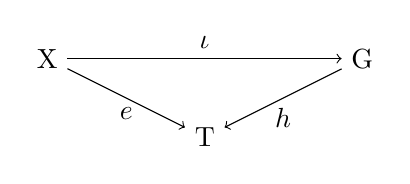
\begin{tikzpicture}
                \node (a) at (0,0) {X};
                \node (c) at (4,0) {G};
                \node (d) at (2,-1) {T};
                \draw[->] (a) -- (d) node [midway,below] {$e$};
                \draw[->] (a) -- (c) node [midway,above] {$\iota$};
                \draw[->] (c) -- (d) node[midway, below] {$h$};
                % \node (d) at (2,-0.5) {=};
            \end{tikzpicture}
    \end{center} 
\end{minipage}
\vspace{1mm}

\noindent Combining the measurements of a morphism provided by all morphism-rulers with the help of a weight function $w$ gives the weight of the morphism (\autoref{def:weight_of_a_morphism_relative_to_a_type_graph}), and the weight of an object is defined as the semiring sum of the weights of all morphisms from the object to the type graph $T$ (\autoref{def:weight_of_an_object_relative_to_a_type_graph}). In this section, we recall the definition of morphism weight and object weight relative to a type graph from~\cite{endrullis2024generalized_icgt}.
\begin{notation}[\cite{endrullis2024generalized_arxiv_v2}] For morphisms \( \alpha : A \to B \), \( \beta : B \to C \), \( \gamma : A \to C \) and $E \subseteq \operatorname{Hom}(A,B)$, define:
    \begin{flalign*}
               \set{ \alpha \star - = \gamma } &\overset{\operatorname{def}}{=} \{ \beta \in \operatorname{Hom}(B, C) \mid \alpha \star \beta = \gamma \}.
   \\
               \set{ - \star \beta = \gamma }  &\overset{\operatorname{def}}{=} \{ \alpha \in \operatorname{Hom}(A, B) \mid \alpha \star \beta = \gamma \}.
   \\
               E \star \beta                   &\overset{\operatorname{def}}{=} \set{ \alpha \star \beta \mid \alpha \in E }.
    \end{flalign*}
   \end{notation} 
\begin{definition}[Morphism measurement]
    \label{def:measurement_of_a_morphism_relative_to_a_morphism_ruler}
    The \emph{measurement} of a morphism \( h:G \to T \) relative to a morphism-ruler \( e: X \to T \), denoted $m_e(h)$, is defined as:
                \(
                m_e(h) 
                    \overset{\operatorname{def}}{=}
                \card{\{- \star h = e\}}
                \)
\end{definition}

Measurements of a morphism \(h: G \to T\) provided by different morphism-rulers can be combined to obtain the weight of the morphism with the help of the weight function. We define the exponentiation operation for elements of the semiring before defining formally the morphism weight.
\begin{notation}[Exponentiation operation] 
    \label{wfs:def:exponentiation}
Let $(S, \oplus, \odot, 0_S, 1_S)$ be a semiring. We define the exponentiation operation for all $x \in S$ and $n \in \mathbb{N}$ by
   $ x^0 \isdef 1_S$ and $x^{n+1} \isdef x^n \odot x$.
\end{notation}
\begin{definition}[Morphism weight]
    \label{def:weight_of_a_morphism_relative_to_a_type_graph}
        Let $\mathcal{T}=(T,\mathbb{E},\mathcal{S},w)$ be a finitary weighted type graph.
         The \textbf{weight of a morphism $h: G \rightarrow T$ relative to a type graph $\mathcal{T}$} is defined as the semiring product of $w(e)^{m_e(h)}$ for all $e \in \mathbb{E}$:
        \[  w_{\mathcal{T}}(h) \overset{\operatorname{def}}{=} \underset{e \in \mathbb{E}}{\bigodot} 
                w(e)^{m_e(h)} \]
\end{definition}
\begin{definition}[Object weight]
    \label{def:weight_of_an_object_relative_to_a_type_graph}
       Let $\mathcal{T}=(T,\mathbb{E},\mathcal{S},w)$ be a finitary weighted type graph. The \textbf{weight of an object \( G \)} is defined as the semiring sum of $w_\mathcal{T}(h)$, for all \( h \in \operatorname{Hom}(G,T) \):
        \[ w_\mathcal{T}(G) \overset{\operatorname{def}}{=} \underset{h \in \operatorname{Hom}(G,T)}{\bigoplus}  w_\mathcal{T}(h) \]
\end{definition}

\begin{example}
    Consider the two morphisms in~\autoref{fig:example:two_weighted_type_graph_morphisms}, illustrated using the visual notation introduced in \autoref{notation:graph_homomorphism}, and the weighted type graph $\mathcal{T}$ from \autoref{wf:example:weighted_type_graph}:
    \begin{figure}[!ht]
        \centering
        \resizebox{0.49\textwidth}{!}{
        \begin{tikzpicture}
          \graphbox{\( L \)}{-50mm}{0mm}{40mm}{39mm}{2mm}{-6mm}{
            \coordinate (o) at (0mm,-10mm); 
            \node[draw,circle] (l1) at ($(o)+(-10mm,0mm)$) {1};
            \node[draw,circle] (l2) at ($(l1)+(2,0)$) {2};
            \node[draw,circle] (l3) at ($(l1) + (1,0)$) {3};
            \draw[] (l1) -- (l3) node[midway,above] {a};
            \draw[] (l3) -- (l2) node[midway,above] {a};
        } 
            \graphbox{$T$}{0mm}{0mm}{40mm}{39mm}{-10mm}{-17mm}{
                \node[draw,circle] (1) at (0,0) {$1\ 2$};
                \node[draw,circle] (2) at (2,0) {3};
                \draw[->] (1) edge[loop above] node[midway, above] {$a^{1}$} (1) ;
                \draw[->] (1) edge[loop below] node[midway, below] {$b^{1}$} (1) ;
                \draw[->] (1) edge[bend left] node[midway, above] {$a^{1}$}  (2)  ;
                \draw[->] (2) edge[bend left] node[midway, below] {$a^{1}$} (1)   ;
            }
            \node () at (-5mm,-15mm) {$\overset{h_{11}^1}{\to}$};
        \end{tikzpicture}
        }
        \resizebox{0.49\textwidth}{!}{
            \begin{tikzpicture}
              \graphbox{\(L\)}{-50mm}{0mm}{40mm}{39mm}{2mm}{-6mm}{
                \coordinate (o) at (0mm,-10mm); 
                \node[draw,circle] (l1) at ($(o)+(-10mm,0mm)$) {1};
                \node[draw,circle] (l2) at ($(l1)+(2,0)$) {2};
                \node[draw,circle] (l3) at ($(l1) + (1,0)$) {3};
                \draw[] (l1) -- (l3) node[midway,above] {a};
                \draw[] (l3) -- (l2) node[midway,above] {a};
            } 
                \graphbox{$T$}{0mm}{0mm}{40mm}{39mm}{-10mm}{-19mm}{
                    \node[draw,circle] (1) at (0,0) {$1\ 2\ 3$};
                    \node[draw,circle] (2) at (2,0) {};
                    \draw[->] (1) edge[loop above] node[midway, above] {$a^{1}$} (1) ;
                    \draw[->] (1) edge[loop below] node[midway, below] {$b^{1}$} (1) ;
                    \draw[->] (1) edge[bend left] node[midway, above] {$a^{1}$}  (2)  ;
                    \draw[->] (2) edge[bend left] node[midway, below] {$a^{1}$} (1)   ;(1)   ;
                }
                \node () at (-5mm,-15mm) {$\overset{h_{11}^2}{\to}$};
            \end{tikzpicture}
            }
            \caption{Two morphisms a weighted type graph}
            \label{fig:example:two_weighted_type_graph_morphisms}
      \end{figure}
    We have $ w_\mathcal{T}(h_{11}^1) = w(e_{13a})^{m_{e_{13a}}(h_{11}^1)} \odot w(e_{31a})^{m_{e_{31a}}(h_{11}^1)} =
     1^1 * 1^1 = 1$ and $
        w_\mathcal{T}(h_{11}^2) 
        % = 1^1 * 1^1 
        = 1$
\end{example}

In certain scenarios, when measuring a morphism $h :G\to T$ relative to a morphism-ruler $e:X \to T$, it is necessary to exclude specific morphisms $\iota :X \to G$. For this reason, for any set \( \Gamma \subseteq \operatorname{Hom}(A, G) \),

\noindent
\begin{minipage}{0.6\textwidth}
    we define $\Gamma'$ as the set consisting of all morphisms \( \iota : X \to G \) admitting morphisms \( \zeta \colon X \to A \) and \( \alpha \in \Gamma \) such that the diagram illustrated on the right is commutative. Formally,  
    \[
    \Gamma' \overset{\operatorname{def}}{=} \left\{ \iota \in \operatorname{Hom}(X, G)~\middle|~\exists \alpha \in \Gamma,~\exists \zeta:X \to A,~\zeta \star \alpha = \iota \right\}. 
    \]
\end{minipage}
\begin{minipage}{0.4\textwidth}
    \hfill 
    % \begin{center}
        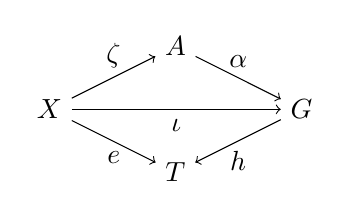
\begin{tikzpicture}[scale=0.8]
            \node (X) at (0,0) {\(X \)};
            \node (A) at (2,1) {\( A \)};
            \node (G) at (4,0) {\( G \)}; 
            \draw[->] (X) -- (A) node[midway, above] {\( \zeta \)};
            \draw[ ->] (X) -- (G) node[midway, below] {\( \iota \)};
            \draw[->] (A) -- (G) node[midway, above] {\( \alpha \)};
            % \node at (2,0.5) {\( = \)};
            \node (T) at (2,-1) {\( T \)};
            \draw[ ->] (X) -- (T) node[midway, below ] {$e$};
            \draw[<-] (T) -- (G) node[midway, below] {$h$};
        \end{tikzpicture}
    % \end{center} 
\end{minipage}

\begin{definition}[Morphism measurement excluding morphisms in a set]
    \label{def:weight_excluding_pre}
    Let \( \Gamma \subseteq \operatorname{Hom}(A, G) \).
    The \emph{measurement} of a morphism \( h:G \to T \) relative to a morphism-ruler \( e: X \to T \), excluding morphisms in \( \Gamma' \), denoted $m_e(h-\Gamma)$, is defined as:
    \[
        m_e(h-\Gamma) \overset{\operatorname{def}}{=} 
            \card{\set{- \star h = e} \setminus \Gamma'}
    \]
\end{definition}
\begin{definition}
    \label{def:weight_excluding}
    Let $\mathcal{T}=(T,\mathbb{E},\mathcal{S},w)$ be a finitary weighted type graph. The \textbf{weight of a morphism $h: G \to T$ relative to a set $\mathbb{E}$ of morphism-rulers excluding morphisms in \( \Gamma' \)} is defined as the semiring product of $w(e)^{w_e(h-\Gamma)}$ for $e \in \mathbb{E}$:
    \[ 
        w_\mathcal{T}(h-\Gamma) \overset{\operatorname{def}}{=} \underset{e \in \mathbb{E}}{\bigodot} 
    w(e)^{m_e(h-\Gamma)}
            \]
\end{definition}


\begin{lemma}[Lemma 4.5~\cite{endrullis2024generalized_arxiv_v4}]
\label{lem:wf:morphism_weight_geq_1_neq_0}
Let $\mathcal{T} = (T, \mathbb{E}, S, \mathbf{w})$ be a finitary weighted type graph. Then
\begin{itemize}
    \item for every $\phi : G \to T$: $1_S \preceq \mathbf{w}_\mathcal{T}(\phi) \neq 0_S$;
    \item for every $\phi : G \to T$ and $\alpha : A \to G$: $1_S \preceq \mathbf{w}_\mathcal{T}(\phi - (\alpha \circ -)) \neq 0_S$;
\end{itemize}
\end{lemma}
\begin{remark}
    \label{rem:wf:weight_of_object_geq_1}
    By Axiom \eqref{wfs:ax:s1}, for all objects \( G \) with $\operatorname{Hom}(G,T)\neq \emptyset$, we have \( 
    w_\mathcal{T}(G) \succeq 1_\mathcal{S} \).
\end{remark}